\documentclass[
  oneside,
  english,
  coorientadorbanca,
  embeddedlogo,
  noabntexcite
]{ufsc-thesis-rn46-2019}

\usepackage[T1]{fontenc} % fontes
\usepackage[utf8]{inputenc} % UTF-8
\usepackage{lmodern}
\usepackage{pdfpages} % Inclui PDF externo (ficha catalográfica)
\usepackage{csquotes}
\usepackage{amsmath}
\usepackage{mathtools}
\usepackage[newfloat]{minted}
\usepackage{graphicx}

\usepackage{paper_alcides}

\usepackage{caption} % configures hyperref to point to top of images
\usepackage{subcaption} % adds subfigures
\usepackage[style=abnt]{biblatex}
\addbibresource{bibliography/llvm.bib}
\addbibresource{bibliography/pratt.bib}
\addbibresource{bibliography/refinements.bib}
\addbibresource{bibliography/thesis.bib}

\usepackage{tikz}
\usetikzlibrary{arrows.meta}
\usetikzlibrary{positioning}
\usetikzlibrary{trees}

\newcommand\myflowchartlowermargin{1.2cm}

\newcommand{\bnfvar}[1]{\ \bnfvars{#1}}
\newcommand{\bnfvars}[1]{\langle\textrm{#1}\rangle}
\newcommand{\bnfter}[1]{\;\bnfters{#1}}
\newcommand{\bnfters}[1]{\textrm{`}\textrm{#1}\textrm{'}}
\newcommand{\bnfor}[1]{\;\mid{} #1}
\newcommand{\bnfprod}[2]{\bnfvars{#1} &\ &::= & #2}
\newcommand{\bnfmore}[1]{ && \mid{} & #1}

\newcommand{\token}[1]{$\langle\textrm{#1}\rangle$}

%%%%%%%%%%%%%%%%%%%%%%%%%%%%%%%%%%%%%%%%%%%%%%%%%%%%%%%%%%%%%%%%%%%%
%%% Configurações da classe (dados do trabalho)                  %%%
%%%%%%%%%%%%%%%%%%%%%%%%%%%%%%%%%%%%%%%%%%%%%%%%%%%%%%%%%%%%%%%%%%%%

% Informações para capa e folha de rosto/certificacao

% Caso o título contenha alguma porção LaTeX ilegível, defina um título
% alternativo opcional com []'s para ser usado no campo Title do PDF
% IMPORTANTE: Os títulos deveriam ser iguais. Apenas use um título
% alternativo se o título não puder ser expresso com letras e números
\titulo{A programming language with refinement types and its LLVM-IR front end implementation.}

\autor{Bernardo Ferrari Mendonça}
\data{24 de Fevereiro de 2022} % ou \today
\instituicao{Universidade Federal de Santa Catarina}
\centro{Centro Tecnológico}
\local{Florianópolis} % Apenas cidade! Sem estado
\programa{Programa de Graduação em Ciência da Computação}
% Os dois próximos itens são usados para gerar o \preambulo
%\tese % ou \dissertacao ou \tcc
%\titulode{doutor em Ciência da Computação}

%%% Atenção! No caso de TCC, além de usar \tcc, outros comandos devem ser fornecidos:
%%%
\tcc{}
\departamento{Departamento de Informática e Estatística}
\curso{Ciência da Computação}
\titulode{Bacharel em Ciência da Computação}
% %% Para TCCs, orientadores e coorientadores podem ser externos, logo a
% %% BU exige que sua afiliação seja explicitada. Por padrão, assume-se
% %% UFSC. Você pode alterar a afiliação com os comandos abaixo:

% Orientador, coorientador, membros da banca e coordenador
% As regras da BU agora exigem que Dr. apareça **depois** do nome
% Dica: para gerar Profᵃ. use Prof\textsuperscript{a}.
% Dica 2: para feminino use \orientadora e \coorientadora
\orientadorext{Prof.\ Alcides Miguel Cachulo Aguiar Fonseca, Dr.}{Universidade de Lisboa}
\coorientadorext{Prof.\ Rafael de Santiago, Dr.}{Universidade Federal de Santa Catarina}
\membrabanca{Prof\textsuperscript{a}. Jerusa Marchi, Dr.}{Universidade Federal de Santa Catarina}
% Dica: se feminino, \coordenadora
\coordenador{Prof.\ Jean Everson Martina, Dr.}

\begin{document}

%%%%%%%%%%%%%%%%%%%%%%%%%%%%%%%%%%%%%%%%%%%%%%%%%%%%%%%%%%%%%%%%%%%%
%%% Principais elementos pré-textuais                            %%%
%%%%%%%%%%%%%%%%%%%%%%%%%%%%%%%%%%%%%%%%%%%%%%%%%%%%%%%%%%%%%%%%%%%%

% Inicia parte pré-textual do documento capa, folha de rosto, folha de
% aprovação, aprovação, resumo, lista de tabelas, lista de figuras, etc.
\pretextual{}
\imprimircapa{}
\imprimirfolhaderosto*
% Atenção! \cleardoublepages são inseridos automaticamente
% Atenção! esse \protect é importante
\protect{}%\incluirfichacatalografica{ficha.pdf}
\imprimirfolhadecertificacao{}

% Listas de "coisas". O * no final faz com que as listas não sejam
% incluídas como entratas do sumário (\tableofcontents)

% \listoftables*
% \listofalgorithms*
% \listoffigures*
% \tableofcontents*

\begin{dedicatoria}
  This work is dedicated to my mother, Marcela Ferrari, my sister Camila Ferrari, and to my grandparents Márcio Ferrari and Cláudia Ferrari who plowed the field where I bloom.
\end{dedicatoria}

\begin{agradecimentos}
  TODO ack
\end{agradecimentos}

\begin{epigrafe}
  TODO epigrafe
\end{epigrafe}

\begin{resumo}[Resumo]
  TODO Resumo

  % Atenção! a BU exige separação através de ponto (.). Ela recomanda de 3 a 5 keywords
  \vspace{\baselineskip}
  \textbf{Palavras-chave:} linguagem de programação\@. tipos refinados\@. representação intermediária de código\@. compilador\@. LLVM\@. LLVM-IR\@.
\end{resumo}

\begin{abstract}
  TODO abstract

  \vspace{\baselineskip}
  \textbf{Keywords:} Keyword. Another Compound Keyword. Bla.
\end{abstract}

\listoffigures*  % O * evita que apareça no sumário

% \begin{listadesimbolos}
%   \($1\)   & Atribuição \\
%   \($1\)   & Quantificação existencial \\
%   $\rightarrow$   & Implicação \\
%   $\wedge$   & E lógico \\
%   $\vee$   & Ou lógico \\
%   $\neg$   & Negação lógica \\
%   $\mapsto$   & Mapeia para \\
%   $\sqsubseteq$   & Subclasse (em ontologias) \\
%   $\subseteq$   & Subconjunto: $\forall x\;.\; x \in A \rightarrow x \in B$ \\
%   $\langle\ldots\rangle$ & Tupla \\
%   $\forall$   & Quantificação universal \\
%   mmmmm & Nenhum sentido, apenas estou aqui para demonstrar a largura máxima dessas colunas. Ao abrir o ambiente \texttt{listadesimbolos}, pode-se fornecer um argumento opcional indicando a largura da coluna da esquerda (o default é de 5em): \texttt{\textbackslash{}begin\{listadesimbolos\}[2cm] .... \textbackslash{}end\{listadesimbolos\}} \\
% \end{listadesimbolos}

\tableofcontents*

%%%%%%%%%%%%%%%%%%%%%%%%%%%%%%%%%%%%%%%%%%%%%%%%%%%%%%%%%%%%%%%%%%%%
%%% Corpo do texto                                               %%%
%%%%%%%%%%%%%%%%%%%%%%%%%%%%%%%%%%%%%%%%%%%%%%%%%%%%%%%%%%%%%%%%%%%%
\textual{}

\chapter{Introduction}\label{chapter:introduction}

As stated by~\textcite{Aho:2006:CPT:1177220}, \textquote{Programming languages are notations to describe computations to people and to machines}.
These notations can take numerous forms.
They range from lower-level languages, such as machine code ready to be executed by a specific machine, to a higher-level language, such as C, Java, Rust, Haskell and Ml.
Lower-level languages like machine code are very verbose in how they describe computations; usually describing directly to the machine when and how to execute each computation through simple notations like: add the values from two data locations, compare two value, jump the next 4 instructions, and so on~\cite{Aho:2006:CPT:1177220}.
Whereas, in a higher-level language, we can describe computations in a more abstract set of notations, such as functions and types, without needing to expose details from the specific machine that will execute them~\cite{Aho:2006:CPT:1177220}.
Hence, using a higher-level programming languages eases how people can describe computations to machines and to one another~\cite{Aho:2006:CPT:1177220}.
However, in order to translate a higher-lever programming language to machine code capable of running on a machine's processor, we need to design and build programs called compilers~\cite{Aho:2006:CPT:1177220}.

A compiler is a program that receives as input a program written in a \textit{source} language and translates it to a semantically equivalent program written in a \textit{target} language
~\cite{Aho:2006:CPT:1177220}.
This is what enables us to write programs in higher-level languages that are able to execute at a machine's processor.
A program written with a higher-level language such as C is fed into a compiler like Clang, then Clang translates the provided source program to a program in a target language, like Intel's x86 processor's machine code, ready to be executed.
During the translation process between the \textit{source} and \textit{target} languages, the compiler goes through two major execution steps: the analysis step, and the synthesis step~\cite{Aho:2006:CPT:1177220}.
The analysis step, called the compiler's \textit{front end}, organizes the information included in the source program into a grammatical structure, and then uses this grammatical structure, together with some metadata collected during its construction, to build what is called an intermediate representation~\cite{Aho:2006:CPT:1177220}.
Furthermore, the synthesis step, called the compiler's \textit{back end}, uses this intermediate representation to compute the desired target program~\cite{Aho:2006:CPT:1177220}.

Though it is possible to build a compiler that translates directly to a target machine code, this hinders portability and modularity~\cite{appel2003modern}.
Suppose we wish to implement a compiler for the source language $i$ to the target machine language $j$, we can implement just the compiler's \textit{front end} for $i$ and use a proven working \textit{back end} for $j$~\cite{Aho:2006:CPT:1177220}.
Therefore, if we wish to implement compilers for $n$ different programming languages to $m$ different machine languages, we can avoid building $n \times m$ compilers building $n$ \textit{front ends} and $m$ \textit{back ends}~\cite{Aho:2006:CPT:1177220}.

If we give the analysis-synthesis model of a compiler a more fine-grained look, we can identify that the compiler's front and back end operate as a series of phases, each one transforming one intermediate representation to another in order to further advance the computation of the target program~\cite{Aho:2006:CPT:1177220}.
The analysis step, or front end, may be subdivided into: a lexical analyzer, a syntax analyzer, a semantic analyzer and an intermediate code generator; also, the synthesis step may be subdivided into: machine-independent code optimization, code generation, and machine-dependent code optimization~\cite{Aho:2006:CPT:1177220}.
The different phases and the intermediate representations between them can be seen at Figure~\ref{figure:compilation-phases}.

\begin{figure}[!ht]
  \centering
  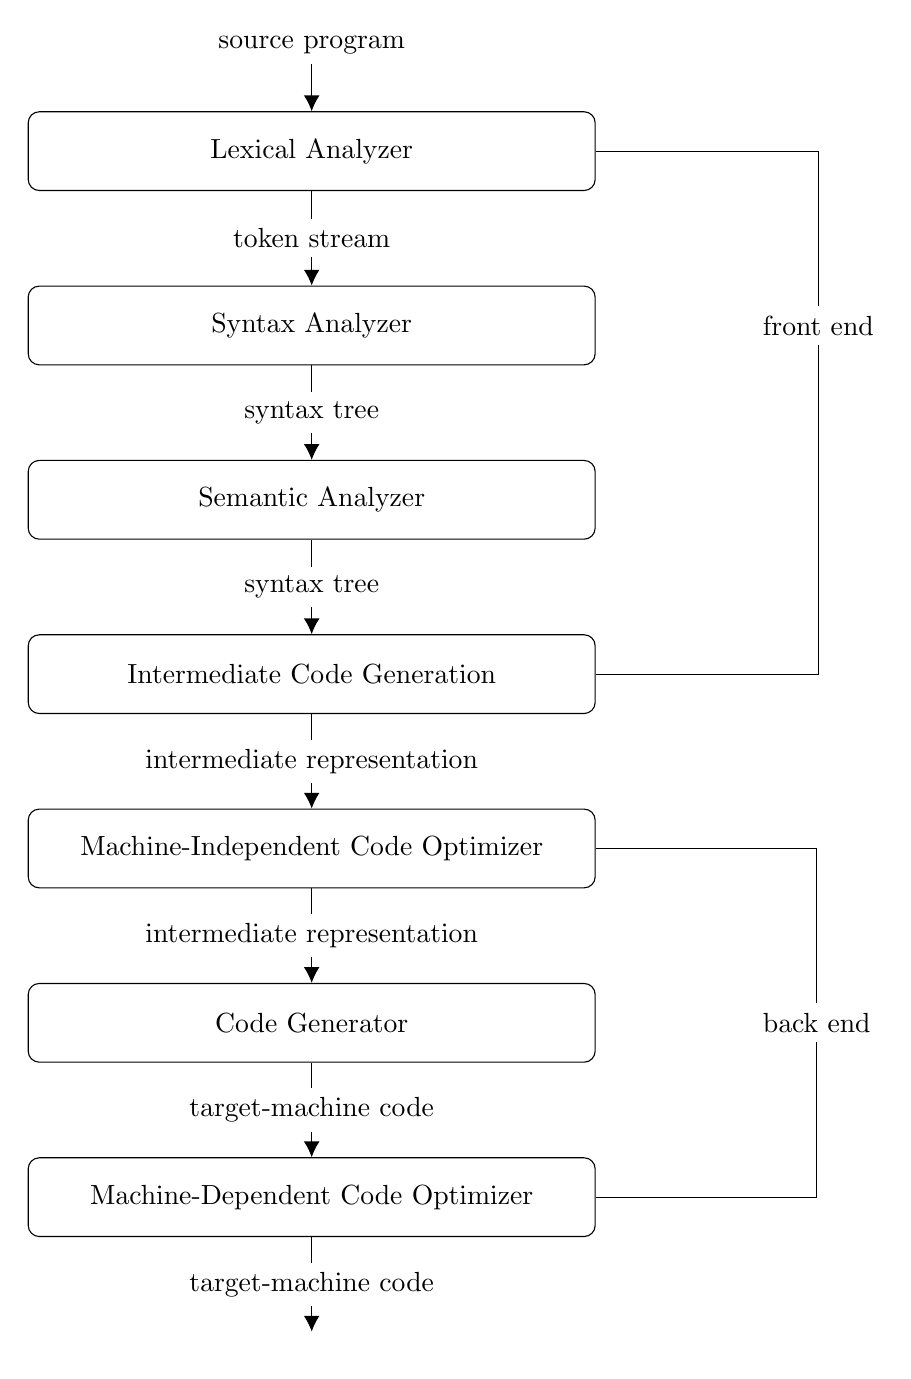
\begin{tikzpicture}[
    >={Latex[width=2mm, length=2mm]},
    ir/.style = {
        fill=white
      },
    phase/.style = {
        rectangle,
        rounded corners,
        minimum width=7.2cm,
        minimum height=1cm,
        text centered,
        draw=black,
      },
    ]
    \node (start) [ir] {source program};
    \node (lexical) [phase, below=\myflowchartlowermargin/2 of start] {Lexical Analyzer};
    \node (syntax) [phase, below=\myflowchartlowermargin of lexical] {Syntax Analyzer};
    \node (semantic) [phase, below=\myflowchartlowermargin of syntax] {Semantic Analyzer};
    \node (intermediate) [phase, below=\myflowchartlowermargin of semantic] {Intermediate Code Generation};
    \node (opt ind) [phase, below=\myflowchartlowermargin of intermediate] {Machine-Independent Code Optimizer};
    \node (codegen) [phase, below=\myflowchartlowermargin of opt ind] {Code Generator};
    \node (opt dep) [phase, below=\myflowchartlowermargin of codegen] {Machine-Dependent Code Optimizer};
    \node (end) [below=\myflowchartlowermargin of opt dep] {};

    \node (frontend) [right=2cm of syntax] {front end};
    \node (backend) [right=2cm of codegen] {back end};

    \draw [->] (start) -- (lexical);
    \draw [->] (lexical) -- node [ir] {token stream} (syntax);
    \draw [->] (syntax) -- node [ir] {syntax tree} (semantic);
    \draw [->] (semantic) -- node [ir] (syntax tree) {syntax tree} (intermediate);
    \draw [->] (intermediate) -- node [ir] {intermediate representation} (opt ind);
    \draw [->] (opt ind) -- node [ir] {intermediate representation} (codegen);
    \draw [->] (codegen) -- node [ir] {target-machine code} (opt dep);
    \draw [->] (opt dep) -- node [ir] {target-machine code} (end);
    \draw (lexical.east) -| (frontend.north);
    \draw (intermediate) -| (frontend);
    \draw (opt ind.east) -| (backend.north);
    \draw (opt dep.east) -| (backend);
  \end{tikzpicture}
  \caption{Phases of a compiler and the intermediate representations between them. Adapted from~\textcite{Aho:2006:CPT:1177220}.}\label{figure:compilation-phases}
\end{figure}

According to \textcite{appel2003modern}, \textquote{An intermediate representation (IR) is a kind of abstract machine language that can express the target-machine operations without committing to too much machine-specific detail}.
The authors continue by adding that the IR \textquote{is also independent of the details of the source language}~\cite{appel2003modern}.
This means that the abstract notations exclusive to a higher-level language are handled by the front end of a compiler so that, by the time the source program is transformed into the IR, the computations described by the IR are semantic equivalent to the computations described by the source program but are now in the notations of an abstract machine language.
Although the semantics of the computations are the same, there may be semantics in the higher-level language that are not present in the IR.\@
The front end of a compiler is then responsible to check if all semantic aspects of the source program are sound to the source language specifications before the generation of the IR~\cite{Aho:2006:CPT:1177220}.
The authors explain that the checks made during compilation are called \textit{Static Checks}, and they are not only capable of assuring that the source program can be successfully compiled, but have the potential to catch programming errors early, before the program can be executed~\cite{Aho:2006:CPT:1177220}. One of the static checks executed during compilation is \textit{type checking} and is part of the semantic analysis phase of the compiler's front end~\cite{appel2003modern}.

The type checking executed during the semantic analysis phase is designed in accordance with the source language's type system.
\textcite{pierce2002types} defines a type system as: \textquote{A tractable syntactic method for proving the absence of certain program behaviors by classifying phrases according to the kinds of values they compute}.
Hence, a phrase written with higher-level notations such as
\begin{equation}\label{eq:type_example1}
  \verb+x * 30+
\end{equation}
may be classified to compute a value of type \verb+Integer+, written
\begin{equation*}
  \verb+x * 30: Integer+
\end{equation*}
meaning that~\ref{eq:type_example1} is a phrase that computes a mathematical integer value.
As a counter example, if defined by the type system that the multiplication between a value of type \verb/Character/ and a value of type \verb/Integer/ was not allowed, and we had both classifications
\begin{equation*}
  \verb/x: Character/ \quad \textrm{and} \quad \verb/30: Integer/
\end{equation*}
the phrase in~\ref{eq:type_example1} would be semantically unsound and should be indicated as a type error by the type checker.

According to \textcite{jhala2020tutorial} type systems are mainly used to describe valid sets of values that can be used for different computations, so that the compiler can eliminate, during its execution, a variety of possible run-time errors during the target program execution.
Type systems like the ones used by popular modern programming languages such as C\#, Haskell, Java, OCaml, Rust and Scala have similar kinds of rules and are the most widespread tool used to guarantee the correct behavior of a program~\cite{jhala2020tutorial}.
\textcite{jhala2020tutorial} affirm that, although type systems are widespread and effective, well-typed programs do go wrong; and the authors goes on to describe a few wrong behaviors that are common to the most popular type systems. Within them, we have:
\begin{itemize}
  \item \textbf{Division by zero:} Constraining the types of the division operation to \verb/int/ does not protect the program to execute a division by zero at run-time; also, it does not guarantee that the arithmetic operations will not under- or over-flow~\cite{jhala2020tutorial}.
  \item \textbf{Buffer overflow:} Constraining the index of the access of a \verb/array/ or \verb/string/ to \verb/int/ does not protect the program to try to access data from beyond the data structure's end~\cite{jhala2020tutorial}.
\end{itemize}

An effort can be made while designing a type system so that they can further restrict the values of certain types.
We can extend a type system to further \textit{refine} its types with logic predicates and this method is called \textit{Refinement types with predicates}~\cite{jhala2020tutorial}.
It allows programmers to constrain existing types by using predicates to assert desired properties of the values they want to describe~\cite{jhala2020tutorial}.
For example, while \verb/int/ types can assume any integer values, we can write the refined type
\begin{equation*}
  \verb/type nat = {v:int | 0 <= v}/
\end{equation*}
where the newly defined type \texttt{nat} will only be able to assume positive integer values.
Alone, this refinements may seam a just a gimmick, but combined with function the programmer can describe precise contracts that describe the functions legal inputs and outputs~\cite{jhala2020tutorial}.
For example, the author of an \texttt{array} library may specify the functions signatures types
\begin{equation*}
  \begin{aligned}
     & \verb/fn size: x:array(a) -> {v:nat | v = length(x)}/      \\
     & \verb/fn  get: x:array(a) -> {v:nat | v < length(x)} -> a/ \\
  \end{aligned}
\end{equation*}
where \verb!size! and \verb!get! are functions and \verb!x! is the name of the first variable.
In this type system, a call to \verb+size(arr)+ returns a value $s$ of type \verb!nat! constrained to a single value equal to the length of \verb!arr!; hence, the type of $s$ constrains $s$ to the exact length of \verb+arr+.
Furthermore, a call to \verb+get(arr, i)+ requires the index \verb+i+ to be within the bounds of \verb+arr+.
Given these definitions, the refinement type checker can then prove, during the analysis phase (i.e.\ at compile-time), that the contracts of both \verb+size+ and \verb+get+ will not be violated, ensuring all array access to be sated when executing the target program (i.e.\ at run-time).

\section{Motivation and research problem}

There is an increasing number of uses of refinement types being implemented on top of existing languages.
For example: the work of~\textcite{vazou2014liquidhaskell} presenting LiquidHaskell as refinement types for the Haskell language; the work of~\textcite{vekris2016refinementtypescript} integrating refinement types for the TypeScript language; the work of~\textcite{sammler2021refinedc} integrating refinement types for the C language; and, the work of~\textcite{vazou2018refinementruby} integrating refinement types for the Ruby language.

Although refinement types have been proved useful in improving the static checking capabilities of higher level languages, there is a lack of research on bringing refinement types to the intermediate code generation phase of a compiler's front end.
Hence, we state the research problem in the form of the question: `What can we discover when we add refinement types to the intermediate code generation phase of a compiler's front end?'.

\section{Goals}\label{chapter:introduction:sec:goals}

The primary goal of this work is to discuss and validate the following thesis: A front-end for a higher-level language with refinement types can make use of refinement types to allow optimizations opportunities during intermediate code generation not present in higher-level languages without refinement types.

For allowing this discussion, we will be designing a language with refinement types called \textit{Ekitai} and implementing its front end.
Designing a new language is particularly advantageous because we have full control of all the language features being implemented and allow us to incrementally design the language, the refinement type system, and the intermediate code generation, one feature at a time.

\subsection{Specific Goals}\label{chapter:introduction:sec:goals:specific_goals}
The specific research artifacts constructed by this work that allow the discussion of the thesis are:
\begin{itemize}
  \item The specification of \textit{Ekitai's} lexical elements;
  \item The specification of \textit{Ekitai's} syntax;
  \item The specification of \textit{Ekitai's} type system with refinement types;
  \item The implementation of \textit{Ekitai's} front end including:
        \begin{itemize}
          \item A lexical analyzer;
          \item A syntactic analyzer;
          \item A semantic analyzer with a type checker;
          \item An intermediate code generator;
        \end{itemize}
  \item The implementation of optimizations during intermediate code generation.
\end{itemize}

\section{Methodology}

The aim of this work is to find optimizations opportunities during intermediate code generation of a higher-level language with refinement types.
In order to achieve the specific goals specified in Section~\ref{chapter:introduction:sec:goals:specific_goals} we will employ different methods during research.

In the specification of the \textit{Ekitai} programming language aspects we will employ techniques from the established literature, such as books and articles, on language design and compiler construction.
Also, in order to specify the type system with refinement types we analyze the recent publications about refinement types in the ACM Sigplan's conferences and journals.
Whereas in the implementation of \textit{Ekitai's} front end we will develop a front end using the Rust programming language employing techniques from the established literature, such as books and articles, and from open-source implementations of modern industry programming language compilers and tools.

\section{Structure of the work}

In the next chapter, Chapter~\ref{chapter:background}, we will introduce the background knowledge needed to design a higher level language's front end. Furthermore, in Chapter~\ref{chapter:related_work}, we explore other pieces of work from articles and industry that are tangent to our goal. Then, in Chapter~\ref{chapter:proposal}, we describe the proposed \textit{Ekitai} language.

\chapter{A review on front end design and implementation}\label{chapter:background}

In this chapter we present a brief review of the background needed to build a compiler's front end.
We begin by presenting what is a lexical analyzer and how it is constructed in Section~\ref{chapter:background:sec:lexical}.
We continue by presenting the aspects of a syntax analyzer in Section~\ref{chapter:background:sec:syntax}.
Furthermore, we go on to explore the semantic analyzer and the tools used to formalize the type system in Section~\ref{chapter:background:sec:semantic}.
And then explore the aspects of intermediate code generation in Section~\ref{chapter:background:sec:intermediate}.

\section{Lexical Analysis}\label{chapter:background:sec:lexical}

The first phase of a compiler is called lexical analysis.
The lexical analyzer will read a stream of characters from the source program and group the characters into sequences called \textit{lexemes} according to the \textit{patterns} defined for each \textit{token name}~\cite{Aho:2006:CPT:1177220}.
\textcite{Aho:2006:CPT:1177220} describes that, for each lexeme grouped by reading the input character stream, the lexical analyzer will generate a \textit{token} which constitutes a pair of the token name and some optional metadata, e.g.\ the start and end position of the respective lexeme in the input character stream, written
\begin{equation*}
  \langle \textrm{token name},\ \textrm{metadata}\rangle
\end{equation*}
For example, upon analyzing the following program:
\begin{equation*}
  \verb|let a = b + 60 / c|
\end{equation*}
A lexical analyzer may output the following token stream:
\begin{equation}\label{figure:introduction_token_stream}
  \begin{aligned}
     & \langle \textrm{let},        &  & \{lexeme:\ \texttt{let}, &  & begin: 0,  &  & end: 3\}\rangle  \\
     & \langle \textrm{identifier}, &  & \{lexeme:\ \texttt{a},   &  & begin: 4,  &  & end: 5\}\rangle  \\
     & \langle =,                   &  & \{lexeme:\ \texttt{=},   &  & begin: 6,  &  & end: 7\}\rangle  \\
     & \langle \textrm{identifier}, &  & \{lexeme:\ \texttt{b},   &  & begin: 8,  &  & end: 9\}\rangle  \\
     & \langle +,                   &  & \{lexeme:\ +,            &  & begin: 10, &  & end: 11\}\rangle \\
     & \langle \textrm{number},     &  & \{lexeme:\ \texttt{60},  &  & begin: 12, &  & end: 14\}\rangle \\
     & \langle /,                   &  & \{lexeme:\ /,            &  & begin: 15, &  & end: 16\}\rangle \\
     & \langle \textrm{identifier}, &  & \{lexeme:\ \texttt{c},   &  & begin: 17, &  & end: 18\}\rangle
  \end{aligned}
\end{equation}
In this case, the metadata collected by the analyzer is very pedantic including even redundant data as the lexemes for simple patterns of the token names $=$, $+$ and $/$.
When no metadata is needed it can be omitted from the token notation, e.g. \verb+<{>+.

In order to classify a lexeme to be of a given token name we employ the use of \textit{patterns}.
One of the important notations for the description of token patterns are regular expressions.
They are very effective in specifying the type of patterns usually needed to classify lexemes into tokens and can be used for automatic generation of a lexical analyzer~\cite{Aho:2006:CPT:1177220}.
A simple description of the patterns for the tokens used in the example above can be given by regular expressions with rules of the form $\textit{token name} \rightarrow \textit{regular expression}$ as follows:
\begin{equation*}
  \begin{aligned}
    \textrm{identifier} & \rightarrow \ {[A-Za-z]}^+ \\
    \textrm{number}     & \rightarrow \ {[0-9]}^+    \\
    \textrm{let}        & \rightarrow \ let          \\
    =                   & \rightarrow \  =           \\
    /                   & \rightarrow \ /            \\
    +                   & \rightarrow \ +            \\
  \end{aligned}
\end{equation*}
This rules can then, either be used by lexical analyzer generators to automatically generate a program for lexical analysis, or, be used as the formal specification for handwritten lexers to be based upon~\cite{Aho:2006:CPT:1177220}.

\section{Syntax Analysis}\label{chapter:background:sec:syntax}

The second phase of a compiler is called syntax analysis, or \textit{parsing}.
The \textit{parser} then receives as input a token stream produced by the lexical analyzer and creates a tree-like intermediate representation that is constrained by a particular grammatical structure~\cite{Aho:2006:CPT:1177220}.

If we give the token stream~\eqref{figure:introduction_token_stream} as input to a parser it may produce the \textit{parse tree} structure found on Figure~\ref{figure:introduction_ast}.
This structure has more information than the linear token stream it received as input.
For example, it is prepared in such a way to preserve the order of operations from classic arithmetic.
The tree is composed of two interior nodes labeled $\bnfvars{Expr}$ for binary operations: the bottom one, denoting the sub-expression
\begin{equation*}
  \bnfvar{Expr}_{bottom} = \texttt{60 / c}
\end{equation*}
and the top one, denoting the whole expression
\begin{equation*}
  \bnfvar{Expr}_{top} = \texttt{a +} \bnfvar{Expr}_{bottom} = \texttt{a + 60 / c}
\end{equation*}
This structure makes explicit that we must first evaluate the result of $\bnfvars{Expr}_{bottom}$, dividing $60$ by $c$, before we can evaluate the result of $\bnfvars{Expr}_{top}$, adding $a$ to the result of $\bnfvars{Expr}_{bottom}$.

\begin{figure}[ht]
  \centering
  \begin{tikzpicture}
    \node (is-root) {$\bnfvars{Let}$} [sibling distance=2cm]
    child { node {let} }
    child {
        node {$\bnfvars{Pattern}$}
        child {
            node[align=center] {id}
            child {
                node {a}
                edge from parent[dashed]
              }
          }
        child[missing] {}
      }
    child { node {=} }
    child {
        node {$\bnfvars{Expr}$}
          [sibling distance=1.2cm]
        child {
            node {id}
            child {
                node {b}
                edge from parent[dashed]
              }
          }
        child[missing]{}
        child {
            node {$\bnfvars{Bin-op}$}
            child{ node {$+$} }
            child[missing]{}
          }
        child[missing]{}
        child {
            node {$\bnfvars{Expr}$}
              [sibling distance=2cm]
            child[missing]{}
            child {
                node {number}
                child {
                    node {60}
                    edge from parent[dashed]
                  }
              }
            child {
                node {$\bnfvars{Bin-op}$}
                child {
                    node {$/$}
                  }
              }
            child {
                node {id}
                child {
                    node {c}
                    edge from parent[dashed]
                  }
              }
          }
      };
  \end{tikzpicture}
  \caption{
    A possible parse tree output for the token stream~\eqref{figure:introduction_token_stream}.
    Leafs are shown as the token names from the token stream.
    Here lexemes for non-trivial tokens are appended with dashed lines underneath token names for example purposes.
  }\label{figure:introduction_ast}
\end{figure}

\subsection{Precise definition of context-free grammars and ambiguity}
Every programming language has precise rules that prescribe the correct syntactic structure of its programs and the syntax of such syntactic structure can be described by a context-free grammar~\cite{Aho:2006:CPT:1177220}.
A context-free grammar has four components:
\begin{itemize}
  \item A finite set $\Sigma$ of \textit{terminal} symbols, usually called or tokens, and is composed by the set of token names defined in the lexical aspects of the language~\cite{Aho:2006:CPT:1177220};
  \item A finite set $V$ of \textit{nonterminals}, or \textit{variables}, disjoint from the set of terminals, usually called \textit{syntactic variables}~\cite{Aho:2006:CPT:1177220};
  \item A finite set of \textit{productions}, or \textit{rules}, where each production is of the form
        \begin{equation*}
          \begin{alignedat}{2}
            \bnfprod{Variable}{\ s}
          \end{alignedat}
        \end{equation*}
        where $s \in {(\Sigma \cup V)}^*$, meaning $s$ is a string of zero or more terminals and nonterminals in no specific order~\cite{Aho:2006:CPT:1177220, sipser2012introduction};
  \item A designation of a nonterminal as the \textit{start} of the grammar~\cite{Aho:2006:CPT:1177220}.
\end{itemize}

A simple expression language could have its syntactical structure formalized by the following grammar
\begin{equation}~\label{eq:ambiguous_expr_grammar}
  \begin{alignedat}{2}
    \bnfprod{Expr}{\bnfvar{Expr} \bnfvar{Bin-op} \bnfvar{Expr}}  \\
    \bnfmore{\bnfter{}\bnfvar{Expr}\bnfter{}}                    \\
    \bnfmore{\bnfter{number}}                                    \\
    \bnfmore{\bnfter{id}}                                        \\
    \bnfprod{Bin-op}{\bnfter{+} \bnfor{\bnfter{-}} \bnfor{\bnfter{*}} \bnfor{\bnfter{/}}}
  \end{alignedat}
\end{equation}
where: terminals have the token names between quotes, e.g. $\bnfters{id}$;
nonterminals have the syntactic variables names between $\langle$ and $\rangle$, e.g. $\bnfvars{Expr}$;
productions have the form
\begin{alignat}{2}
  \bnfprod{V}{\ s} \nonumber
\end{alignat}
where $\bnfvars{V}$ is the variable at the \textit{head} of the production and $s$ is the string of terminals and nonterminals at the production's \textit{body};
the designation of the starting variable is done by the variable at the head of the first production, in the example above the starting nonterminal is $\bnfvars{Expr}$.
Furthermore, multiple productions can be abbreviated by using the \textit{or} operator denoted by `$\mid$' turning
\begin{alignat}{2}
  \bnfprod{V}{\ s^1} \nonumber \\
  \bnfprod{V}{\ s^2} \nonumber
\end{alignat}
into
\begin{alignat}{2}
  \bnfprod{V}{\ s^1 \bnfor{s^2}} \nonumber
\end{alignat}

In order to show that a particular sentence is in the language formalized by a context-free grammar, we can perform a derivation~\cite{sipser2012introduction}.
A derivation starts with, first, writing the start variable~\cite{sipser2012introduction}.
Then, second, we choose any variable from the sentence written so far and a production with the same variable as head replacing the chosen variable with the body of the chosen production~\cite{sipser2012introduction}.
Then, we repeat the second step until there is no more variables and the sentence is formed only by terminals~\cite{sipser2012introduction}.

To show that the sentence of token names `$id + number * id$' is present in the language specified by grammar~\eqref{eq:ambiguous_expr_grammar} we can perform multiple different derivations. Starting with the start variable
\begin{equation*}
  \begin{aligned}
     & \bnfvars{Expr}
  \end{aligned}
\end{equation*}
we know there are two binary operations, so we perform a derivation to
\begin{equation*}
  \begin{aligned}
     & \bnfvars{Expr}\bnfvar{Bin-op}\bnfvar{Expr}
  \end{aligned}
\end{equation*}
here we can choose what to derivate first.
Although we could choose any variable from the sentence during derivation, we will stick to leftmost derivations, which mandates that we choose the leftmost variable, highlighted in \textbf{bold}, of the sentence to perform the derivation.
So, we could have the leftmost derivation
\begin{equation}\label{eq:ambiouous_derivation1}
  \begin{aligned}
     & \bnfvars{\textbf{Expr}}                                                         \\
     & \bnfvars{\textbf{Expr}}\bnfvar{Bin-op}\bnfvar{Expr}                             \\
     & \bnfvars{\textbf{Expr}}\bnfvar{Bin-op}\bnfvar{Expr}\bnfvar{Bin-op}\bnfvar{Expr} \\
     & \textit{id}\bnfvar{\textbf{Bin-op}}\bnfvar{Expr}\bnfvar{Bin-op}\bnfvar{Expr}    \\
     & \textit{id}\ + \bnfvar{\textbf{Expr}}\bnfvar{Bin-op}\bnfvar{Expr}               \\
     & \textit{id}\ + \ \textit{number} \ \bnfvar{\textbf{Bin-op}}\bnfvar{Expr}        \\
     & \textit{id}\ + \ \textit{number} \ * \ \bnfvar{\textbf{Expr}}                   \\
     & \textit{id}\ + \ \textit{number} \ * \ \textit{id}
  \end{aligned}
\end{equation}
but, we could also have a second leftmost derivation
\begin{equation}\label{eq:ambiouous_derivation2}
  \begin{aligned}
     & \bnfvars{\textbf{Expr}}                                                  \\
     & \bnfvars{\textbf{Expr}}\bnfvar{Bin-op}\bnfvar{Expr}                      \\
     & \textit{id}\ \bnfvar{\textbf{Bin-op}}\bnfvar{Expr}                       \\
     & \textit{id}\ + \ \bnfvar{\textbf{Expr}}                                  \\
     & \textit{id}\ + \ \bnfvar{\textbf{Expr}}\bnfvar{Bin-op}\bnfvar{Expr}      \\
     & \textit{id}\ + \ \textit{number} \ \bnfvar{\textbf{Bin-op}}\bnfvar{Expr} \\
     & \textit{id}\ + \ \textit{number} \ * \ \bnfvar{\textbf{Expr}}            \\
     & \textit{id}\ + \ \textit{number} \ * \ \textit{id}
  \end{aligned}
\end{equation}
thus, having two leftmost derivations that shows the sentence belongs to the grammar's described language.

A grammar is said to be \textit{ambiguous} if it has a non-unique leftmost or rightmost derivation for any sentence of the language it describes~\cite{Aho:2006:CPT:1177220}.
Therefore, grammar~\eqref{eq:ambiguous_expr_grammar} is clearly ambiguous given derivations~\eqref{eq:ambiouous_derivation1} and~\eqref{eq:ambiouous_derivation2}.
From the parse trees in Figure~\ref{fig:ambiguous_parse_tree} we can visualize that the order of operations differ between the derivations of `$id + number * id$'.
In Figure~\ref{fig:ambiguous_parse_tree_a} we have $(id + number) * id$ and in Figure~\ref{fig:ambiguous_parse_tree_b} we have $id + (number * id)$ which have different mathematical meanings.

\begin{figure}[ht]
  \centering
  \begin{subfigure}[b]{0.4\textwidth}
    \centering
    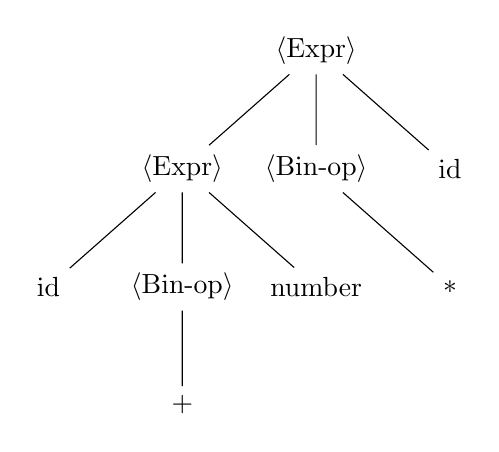
\begin{tikzpicture}
      \node {$\bnfvars{Expr}$} [sibling distance=1.7cm]
      child {
          node {$\bnfvars{Expr}$}
          child {
              node {id}
            }
          child {
              node {$\bnfvars{Bin-op}$}
              child{ node {$+$} }
            }
          child {
              node {number}
            }
        }
      child {
          node {$\bnfvars{Bin-op}$}
          child[missing]{}
          child[missing]{}
          child {
              node {$*$}
            }
        }
      child {
          node {id}
        };
    \end{tikzpicture}
    \caption{Parse tree from derivation~\eqref{eq:ambiouous_derivation1}.}\label{fig:ambiguous_parse_tree_a}
  \end{subfigure}
  \qquad
  \qquad
  \begin{subfigure}[b]{0.4\textwidth}
    \centering
    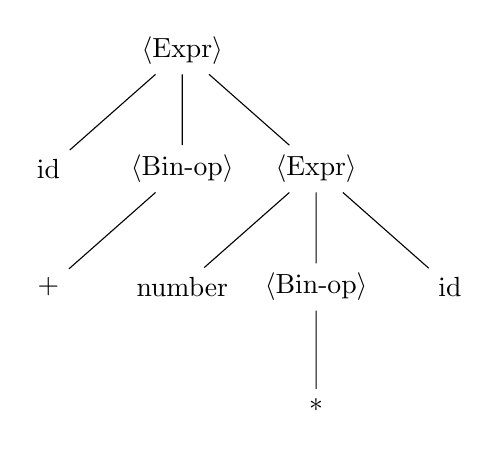
\begin{tikzpicture}
      \node (is-root) {$\bnfvars{Expr}$} [sibling distance=1.7cm]
      child { node {id} }
      child {
          node {$\bnfvars{Bin-op}$}
          child {
              node {$+$}
            }
          child[missing]{}
          child[missing]{}
        }
      child {
          node {$\bnfvars{Expr}$}
          child {
              node {number}
            }
          child {
              node {$\bnfvars{Bin-op}$}
              child{ node {$*$} }
            }
          child {
              node {id}
            }
        };
    \end{tikzpicture}
    \caption{Parse tree from derivation~\eqref{eq:ambiouous_derivation2}.}\label{fig:ambiguous_parse_tree_b}
  \end{subfigure}
  \caption{
    Visual representation of derivations~\eqref{eq:ambiouous_derivation1} and~\eqref{eq:ambiouous_derivation2} in its parse tree form.
  }\label{fig:ambiguous_parse_tree}
\end{figure}

Compilers use parse trees to derive meaning and, therefore, ambiguous grammars are problematic for compilling~\cite{appel2003modern}.
If we were to use some parsing generator algorithm, such as $LL$, $LR$ and their variants, an effort should be made to transform such ambiguous grammars into unambiguous grammars.
As an example, we can present an unambiguous grammar relative to the grammar~\eqref{eq:ambiguous_expr_grammar} as
\begin{equation}~\label{eq:unambiguous_expr_grammar}
  \begin{alignedat}{2}
    \bnfprod{Expr}{\bnfvar{Expr} \bnfter{+} \bnfvar{Term}} \\
    \bnfmore{\bnfvar{Expr}\bnfter{-}\bnfvar{Term}} \\
    \bnfmore{\bnfvar{Term}} \\
    \bnfprod{Term}{\bnfvar{Term} \bnfter{*} \bnfvar{Factor}} \\
    \bnfmore{\bnfvar{Term}\bnfter{/}\bnfvar{Factor}} \\
    \bnfprod{Factor}{\bnfter{(}\bnfvar{Expr}\bnfter{)}} \\
    \bnfmore{\bnfter{number}} \\
    \bnfmore{\bnfter{id}}
  \end{alignedat}
\end{equation}
which, by adding new variables to the grammar, can express unambiguously in its parse trees that: the operators $*$ and $/$ \textit{binds tighter}, or have a \textit{higher precedence}, then $+$ and $-$; and, the operators of the same \textit{binding power}, or \textit{precedence}, are left associative.

\subsection{Review of top-down and bottom-up parsers}
There are two main categories of parser.
First we have parsers that try to construct the parse tree by finding a leftmost derivation starting from the root and creating the nodes of the parse three in preorder, called \textit{top-down} parsers~\cite{Aho:2006:CPT:1177220}.
And second we have parsers that try to construct the parse tree beginning at the leaves and working up to the root by construction a rightmost derivation in reverse by applying a series of reductions on the input stream~\cite{Aho:2006:CPT:1177220}.

Top-down parsers, also called recursive descent parsers, have the advantage of its algorithms being simple enough to be used to construct parsers by hand~\cite{appel2003modern}.
Although simple, classic implementations of recursive descent parsers, such as the $LL(1)$ and $LL(k)$ predictive parsers, cannot deal with ambiguous grammars and, since they rely on leftmost derivations, cannot deal with left recursions on grammar productions~\cite{Aho:2006:CPT:1177220}.
There may also be the need to run a left factoring algorithm in order to generate a correct predictive parsing table for $LL(1)$ and $LL(k)$ automatic parser generators~\cite{Aho:2006:CPT:1177220}.

A non left recursive, left factored grammar for grammar~\eqref{eq:unambiguous_expr_grammar} can be built as
\begin{alignat}{2}
  \bnfprod{Expr}{\bnfvar{Term} \bnfvar{Expr2}}              \label{eq:fat_expr_grammar_expr}  \\
  \bnfprod{Expr2}{\bnfter{+}\bnfvar{Term} \bnfvar{Expr2}}   \label{eq:fat_expr_grammar_expr2} \\
  \bnfmore{\bnfter{-}\bnfvar{Term}\bnfvar{Expr2}}           \nonumber                         \\
  \bnfmore{\ \epsilon}                                      \nonumber                         \\
  \bnfprod{Term}{\bnfvar{Factor} \bnfvar{Term2}}            \label{eq:fat_expr_grammar_term}  \\
  \bnfprod{Term2}{\bnfter{*}\bnfvar{Factor} \bnfvar{Term2}} \label{eq:fat_expr_grammar_term2} \\
  \bnfmore{\bnfter{/}\bnfvar{Factor}\bnfvar{Term2}}         \nonumber                         \\
  \bnfmore{\ \epsilon}                                      \nonumber                         \\
  \bnfprod{Factor}{\bnfter{(}\bnfvar{Expr}\bnfter{)}}       \label{eq:fat_expr_grammar_fact}  \\
  \bnfmore{\bnfter{number}}                                 \nonumber                         \\
  \bnfmore{\bnfter{id}}  \nonumber
\end{alignat}
This grammar complies with every constraint imposed by a classic implementation of a predictive recursive descent parser since it is unambiguous, free of left recursions and left factored.
An example implementation of predictive parsers for the variables $\bnfvars{Expr}$, $\bnfvars{Expr2}$, $\bnfvars{Term}$, $\bnfvars{Term2}$ and $\bnfvars{Factor}$ can be found respectively at Figures~\ref{fig:predictive_parser_expr},~\ref{fig:predictive_parser_expr2},~\ref{fig:predictive_parser_term},~\ref{fig:predictive_parser_term2} and~\ref{fig:predictive_parser_fact}.

\begin{figure}[ht]
  \centering
  \begin{subfigure}[b]{0.48\textwidth}
    \begin{minipage}{\textwidth}
      \begin{minted}[breaklines, linenos, fontsize=\footnotesize]{rust}
fn parse_Expr(p: Parser) -> Parse {
  let t = parse_Term(p);
  let e2 = parse_Expr2(p);
  Expr(t, e2)
}
      \end{minted}
    \end{minipage}
    \caption{}\label{fig:predictive_parser_expr}
  \end{subfigure}
  \quad
  \begin{subfigure}[b]{0.48\textwidth}
    \begin{minipage}{\textwidth}
      \begin{minted}[breaklines, linenos, fontsize=\footnotesize]{rust}
fn parse_Expr2(p: Parser) -> Parse {
  if p.at("+") | p.at("-") {
    p.eat_token();
    let t = parse_Term(p);
    let e2 = parse_Expr2(p);
    Expr2(t, e2)
  } else {
    Empty
  }
}
      \end{minted}
    \end{minipage}
    \caption{}\label{fig:predictive_parser_expr2}
  \end{subfigure}
  \caption{
    Predictive parsers for variables $\bnfvars{Expr}$ (a), and $\bnfvars{Expr2}$ (b), from examples~\eqref{eq:fat_expr_grammar_expr} and~\eqref{eq:fat_expr_grammar_expr2}.
  }\label{fig:predictive_parser_expr_all}
\end{figure}

\begin{figure}[ht]
  \centering
  \begin{subfigure}[b]{0.48\textwidth}
    \begin{minipage}{\textwidth}
      \begin{minted}[breaklines, linenos, fontsize=\footnotesize]{rust}
fn parse_Term(p: Parser) -> Parse {
  let f = parse_Factor(p);
  let t2 = parse_Term2(p);
  Term(f, t2)
}
      \end{minted}
    \end{minipage}
    \caption{}\label{fig:predictive_parser_term}
  \end{subfigure}
  \quad
  \begin{subfigure}[b]{0.48\textwidth}
    \begin{minipage}{\textwidth}
      \begin{minted}[breaklines, linenos, fontsize=\footnotesize]{rust}
fn parse_Term2(p: Parser) -> Parse {
  if p.at("*") | p.at("/") {
    p.eat_token();
    let f = parse_Factor(p);
    let t2 = parse_Term2(p);
    Term2(f, t2)
  } else {
    Empty
  }
}
      \end{minted}
    \end{minipage}
    \caption{}\label{fig:predictive_parser_term2}
  \end{subfigure}
  \caption{
    Predictive parsers for variables $\bnfvars{Term}$ (a), and $\bnfvars{Term2}$ (b), from examples~\eqref{eq:fat_expr_grammar_term} and~\eqref{eq:fat_expr_grammar_term2}.
  }\label{fig:predictive_parser_expr_term_all}
\end{figure}

\begin{figure}[ht]
  \centering
  \begin{minipage}{0.5\textwidth}
    \begin{minted}[breaklines, linenos, fontsize=\footnotesize]{rust}
fn parse_Factor(p: Parser) -> Tree {
  if p.at("(") {
    p.eat_token();
    let expr = parse_Expr(p);
    p.expect(")");
    Expr(expr)
  } else if p.at("id") {
    let token = p.eat_token();
    Id(token)
  } else if p.at("number") {
    let token = p.eat_token();
    Number(token)
  } else {
    panic!("Parse error.");
  }
}
    \end{minted}
  \end{minipage}
  \caption{
    A predictive parser for variable $\bnfvars{Factor}$ in~\eqref{eq:fat_expr_grammar_fact}.
  }\label{fig:predictive_parser_fact}
\end{figure}

We were once again forced to add new variables to the already unambiguous grammar~\eqref{eq:unambiguous_expr_grammar}.
The transformations added variables without clear meanings, such as $\bnfvars{Expr2}$ and $\bnfvars{Term2}$, further complicating the parse tree.
In order to enrich the capabilities of recursive descendant parsers, advances were made to allow recursive descendant parsers to parse some ambiguous grammars with left recursion without the need to left factoring.
\textcite{pratt1973operatorprecedence} proposed an `top-down operator precedence' approach to parse arithmetic expressions by assigning a total order to tokens using a function for the left and right binding power of tokens in order to uniquely create parse trees of ambiguous left recursive expression grammars.
An example Pratt parser for grammar~\eqref{eq:ambiguous_expr_grammar} is found at Figure~\ref{fig:pratt_parser_expr_grammar}.
Pratt parsers work by combining iteration with recursion.
If we try to parse the sentence `$id_1 + number * id_2$' it:
\begin{itemize}
  \item parses $id_1$ and name its node `left';
  \item then enter the loop and parse $\bnfters{+}$ which have a binding power to the left of $1$ and to the right of $2$;
  \item if it binds to the left stronger than the minimum binding power for continuing we stop and return the left node. In this case it does not since the minimum starts at $0$, and we go on to recursively parse $\bnfters{number}$ which becomes the new left;
  \item the next operator is then $\bnfters{*}$ with binding power $3$ and $4$, this time the left binding power still is not smaller than the minimum of $2$, and we recursively parse $id_2$ which becomes a new left;
  \item now upon trying to parse a new operator we break from the loop and return the node for $id_2$ then we construct a node $\bnfvars{Expr}$ with left, which is $\bnfter{number}$ for this iteration, $*$ and $id_2$;
  \item we then return again with another $\bnfvars{Expr}$ node with left, which now is $id_1$, $+$ and the last returned expression as right side finally forming the parse tree with correct precedence found at Figure~\ref{eq:ambiouous_derivation2}.
\end{itemize}

\begin{figure}
  \centering
  \begin{minipage}{0.7\textwidth}
    \inputminted[breaklines, linenos, fontsize=\footnotesize]{rust}{code/pratt_example.rs}
  \end{minipage}
  \caption{
    A Pratt parser for the ambiguous expression grammar~\eqref{eq:ambiguous_expr_grammar}.
  }\label{fig:pratt_parser_expr_grammar}
\end{figure}

\begin{itemize}
  \item error recovery
  \item syntax directed translation
  \item semantic actions
  \item abstract syntax trees
  \item concrete syntax trees
\end{itemize}

\section{Semantic Analysis}\label{chapter:background:sec:semantic}

The third phase of a compiler is called semantic analysis.
It is responsible to use the tree structure generated by the parser to check if the source program is semantically consistent with the language specification.
An important part of semantic analysis is \textit{type checking} where it will try to validate the program to the language specification's type system.

If we feed a type checker with the tree structure presented on Figure~\ref{figure:introduction_ast}.
It may make use of a symbol table containing the type information of the identifiers `b' and `c' to type check all nodes of the tree for consistency.
Suppose a symbol table that maps the identifier `c' to the type `boolean', written `\verb+c: boolean+', which would compose of the values `true' and `false'.
With this information, the type checker would be able to decide if the operation `\verb+60 / c+' is semantically sound to the language's type system.
Does the language type system specifies as valid to divide a number by a boolean?

If it does, what does it mean to divide the value 60 by `false'?
Maybe, whoever designed the language decided that if the dividend is a value of type number and the divisor is a value of type boolean, it will use some rule to convert the divisor's type to number in order to keep the program semantically sound.
Maybe, the language's type system forbids this behavior and will halt the compilation process with some error message.
These are decisions made when building a language's type system.

To do. Here goes type system theory from Types and programming languages.

\section{Intermediate code generation}\label{chapter:background:sec:intermediate}

As the last phase of a compiler's front end we have the intermediate code generation.

To do. Here goes an introduction of Single Static Assignment intermediate representations.

\chapter{State of the art in front end design}\label{chapter:related_work}

In this chapter we will present prior work related to front end construction, refinement types and the LLVM intermediate representation.


\section{Pratt parsers}

The top-down operator precedence parsing algorithm proposed by~\textcite{pratt1973operatorprecedence}, colloquially called Pratt parsers, are top-down parsers that can avoid the common left recursion problem known to this class of parsers.
It makes use of and two binding powers assigned to expression operator tokens to solve operator precedence without having to remove left recursion from the language's syntax grammar~\cite{pratt1973operatorprecedence}.
This works for solving prefix, infix and postfix expressions and is widely used by production grade compilers and tools including ANTLR4~\cite{Parr13} and Rust Analyzer~\cite{matklad2020prattparsing}.
\textcite{matklad2020challenginglrparsing} argues in favor of Pratt parsers as they can be made with production grade error resilience and that the author finds LR parser generators not suitable for production grade compilers and tools.

% Consider the following grammar productions:
% \begin{quote}
%     \begin{verbatim}
% <Sum> ::= <Sum> + <Int>
%         | <Int>
% \end{verbatim}
% \end{quote}
% And consider naive implementation of a parser for Sum
% \begin{quote}
%     \begin{verbatim}
% fn sum(p: &mut Parser) {
%     ...
%     // Try parse <Sum> ::= <Sum> + <Int>
%     sum(p); // (1)
%     p.expect(PLUS_TOKEN);
%     int(p);

%     // If that fails, try <Sum> ::= <Int>
%     ...
% }
% \end{verbatim}
% \end{quote}
% would recursively try to parse `sum' at (1).
% \textcite{Aho:2006:CPT:1177220} argues that this can be solved by eliminating the left recursion from the grammar or by using more powerful parsing methods of the bottom-up family (e.g. $LR(1)$).
% However, for a handwritten parser
% \begin{quote}
%     \begin{verbatim}
% <Sum> ::= <Sum> + <Int>
% \end{verbatim}
% \end{quote}
% indefinitely and never

\section{Incremental compilation}

To do. Explain how to build an incremental compiler with Salsa. Work in progress.

\section{The Sprite Language}

In the work presented by \textcite{jhala2020tutorial}, the authors implemented a higher level language called \textit{Sprite} iteratively adding refinement type features on top of a subset of the OCaml language.

\section{Refinement types with predicates}

A type system can be extended to further \textit{refine} its types with logic predicates~\cite{jhala2020tutorial}.
In \textcite{jhala2020tutorial}, the authors call this technique \textit{Refinement types with predicates}.
It allows programmers to constrain existing types by using predicates to assert desired properties of the values they want to describe~\cite{jhala2020tutorial}.
Refinement types offer the option to add information to the type system about the invariants and correctness properties a programmer may care about~\cite{jhala2020tutorial}.
It is done in such a way that, if the programmer desires, no refinement needs to be added and can be thought like a typical type system~\cite{jhala2020tutorial}.
On the other hand, programmers can incrementally add refinements to ensure important properties about the source program~\cite{jhala2020tutorial}.
They could begin with basic safety requirements, e.g.\ eliminating division by zero and buffer overflow, or guarantee that a function does not receive a empty collection, and then incrementally add to the specification invariants of custom data types~\cite{jhala2020tutorial}.
Ultimately going all the way to specifying and verifying the correctness of different procedures at compile-time~\cite{jhala2020tutorial}.
By enabling verification on the same language as the programming language, refinement types bridge implementation and prof together~\cite{jhala2020tutorial}.
This approach creates a development cycle were the implementation hits programmers to what properties are important to verify, and the verification hits on how the implementation can be restructured to better express the invariants and enable formal proof~\cite{jhala2020tutorial}.

To do. Work in progress.

\section{The LLVM intermediate representation}

To do. Work in progress.

\chapter{The Ekitai language}\label{chapter:proposal}

In this chapter we will describe the design of the \textit{Ekitai} programming and the implementation of its front end to the LLVM intermediate representation.

\section{The Ekitai's lexer}



\section{The Ekitai's parser}

In order to implement the Ekitai's parser the following
% \begin{bnf}
%     \bnfprod{Source File}{\bnfes{} \bnfor{} \bnfpn{Module Items}}\\
%     \bnfprod{Module Items}{\bnfpn{Module Item} \bnfsp{} \bnfpn{Module Items} \bnfor{}}\\
%     \bnfmore{\bnfpn{Module Item}}\\
%     \bnfprod{Module Item}{\bnfpn{Function Definition} \bnfor{}}\\
%     \bnfmore{\bnfpn{Type Definition}}\\
%     \bnfprod{Type Definition}{\bnfpn{Name} \bnfsp{} \bnfpn{Value Constructor List}}\\
%     \bnfprod{Value Constructor List}{\bnfts{\{} \bnfsp{} \bnfpn{Value Constuctors} \bnfsp{} \bnfts{\}}}\\
%     \bnfprod{Value Constructors}{\bnfpn{Value Constructor} \bnfsp{} \bnfts{,} \bnfsp{} \bnfpn{Value Constructors} \bnfor{}}\\
%     \bnfmore{\bnfpn{Value Constructor} \bnfts{,} \bnfor{}}\\
%     \bnfmore{\bnfpn{Value Constructor}}\\
%     \bnfprod{Value Constructor}{\bnfpn{Name} \bnfsp{} \bnfpn{Constructor Parameter List}}\\
%     \bnfprod{Constructor Parameter List}{\bnfts{(} \bnfpn{Constructor Parameters} \bnfts{)}}\\
%     \bnfprod{Constructor Parameters}{\bnfpn{Type}}
% \end{bnf}

To do. Work in progress.

\section{The Ekitai's type system}

To do. Work in progress.

\section{The Ekitai's LLVM intermediate code generator}

To do. Work in progress.

%%%%%%%%%%%%%%%%%%%%%%%%%%%%%%%%%%%%%%%%%%%%%%%%%%%%%%%%%%%%%%%%%%%%
%%% Elementos pós-textuais                                       %%%
%%%%%%%%%%%%%%%%%%%%%%%%%%%%%%%%%%%%%%%%%%%%%%%%%%%%%%%%%%%%%%%%%%%%

\postextual{}
\printbibliography{}

\end{document}
